\chapter{Convolutional RNNs for Video Semantic Segmentation}\label{sec:video_segmentation}

The previous chapter introduced the task of semantic segmentation, where the
model is requested to produce a semantic mask, i.e. to classify every pixel of
an input image. Rather than presenting the algorithm with a single image, a
variant of the segmentation task called cosegmentation, provides it with
multiple images usually taken at different locations in the same scene
(potentially by different cameras). In this setting the model can exploit the
information that the images potentially share to improve the single image
prediction and consequently improve the global score at the same time.

In many ways, \emph{video segmentation} can be seen as an extreme version of
cosegmentation, where the model is asked to segment multiple frames of a video.
As opposed to cosegmentation, where the images depict the same scene from
different angles and in moments potentially very far away in time, in videos the
images come in a seamless fashion and their correlation through time can be
exploited to increase the performances.

The main problem of this task is that if labeling images for semantic
segmentation is expensive, the time required to label all the frames of a
video is even more dramatic. One typical way to alleviate this issue is to
label only a subset of the frames, either by dropping most of the frames and
providing only a few of them with their corresponding mask, or by providing all
the input frames with only a subset of them annotated. Another way to reduce
the labeling effort is to just label the main subject of each frame or to
reduce the number of classes (to the limit case of foreground/background
separation).

Applying machine learning techniques to this class of problems is challenging
due to the lack of large amounts of labeled data, as well as for the huge
amount of time required to train these kind of models that calls for
non-trivial technological solutions. The time spent on operations that are not
strictly related to training, such as loading and preprocessing the data,
saving the weights on disk, saving samples and generating plots to monitor the
progress of the algorithm, has to be minimized. Another recent trend in this
field is to resort to multi-GPU training, that introduces an almost linear
speedup (up to a certain numbers of GPUs)~\cite{theano2016short,ma2016theano}
but increases the complexity of the algorithm, is often subject to constraints
(e.g., the GPUs might have to be hosted by the same machine or node of a
cluster) and makes debugging much less pleasant in many cases.

\autoref{sec:reseg} analyzed ReSeg~\citep{Visin_2016_CVPR_Workshops}, an
RNN-based model for image semantic segmentation. One of the main strengths of
ReSeg comes from the coupling of fast general-purpose CNN feature extractors
with stateful RNNs able to carry the information extracted by the CNNs through
various steps of computation, showing the effectiveness of RNNs applied to the
spatial domain.

% While in ReSeg RNNs are allowed to move over the spatial dimension of the data
% rather than the temporal one.
This approach can be taken a step further by allowing the RNNs to jointly
process space and time information in videos, by placing the CNNs directly into
the inner computation of the recursive layer. This chapter introduces a novel
architecture that aims to address the task separation traditionally enforced by
the CNN-RNN dichotomy jointly processing the temporal and the spatial
information at each level of the recurrent-convolutional hierarchy.


\section{Motivation}

% Intro
In the last years, Convolutional Neural Networks (CNNs) have been successfully
applied to address many computer vision tasks, such as image
classification~\citep{Krizhevsky2012-alexnet,Simonyan2015,
Szegedy-et-al-arxiv2014} and object detection~\citep{Girshick-et-al-arxiv2013,
Sermanet13overfeat} and their application has become ubiquitous in many well
known and widely used commercial products.

More recently, pixel-wise prediction of still images has enjoyed the attention
of the computer vision community. In contrast to image classification and
object detection this \emph{structured prediction} problem requires each
pixel to be classified, which demands for a more fine detail understanding of
the image, as well as consistency in the prediction. In this domain many
state of the art architectures successfully coupled classification models
trained on ImageNet~\citep{Simonyan14vgg,Szegedy15googlelenet} with various
upsampling strategies in a trainable end-to-end fashion to address the
challenging image segmentation and scene parsing task~\citep[see e.g.,~][]{
long2014fully,noh2015learning}.

The success witnessed on still images has rapidly reached the video domain,
achieving remarkable results in tasks such as video action recognition~\citep{
simonyan2014two,karpathy2014large}, event detection in videos~\citep{
yeung2015end} and video captioning~\citep{yao2015describing}. Along this
direction, some effort has been devoted lately to address the more
challenging task of end to end video semantic segmentation~\citep{Tran16v2v}.

While many computer vision video-related tasks involve predicting only a single
or a few outputs per video, some of them -- such as video semantic
segmentation, change detection and object tracking -- require a per
\emph{temporal "voxel"} prediction. As an analogy to 3D voxels, where a
volumetric pixel (or voxel) is used to describe a local portion of the data
that extends across space in three dimensions, temporal voxels refer to 3D
portions of the data that span over a contiguous two-dimensional space and over
a one-dimensional sequence in the temporal domain.
Works in this direction usually define a fixed {\emph a priori} window on the
temporal dimension to obtain a voxel-wise prediction~\citep{Tran16v2v}.

The most common way to address video related tasks with neural network
approaches is to combine CNNs with RNNs in a sequential fashion, by first
applying a (possibly pre-trained) CNN on each frame and then interpreting the
resulting feature maps in a temporal consistent way by processing them with an
RNN~\cite{Donahue-et-al-arxiv2014,Vinyals-et-al-CVPR2015,Karpathy+Li-CVPR2015,
Venugopalan_2015_ICCV}. While this is an effective way to exploit the temporal
information, the two pipelines don't completely benefit from each other, since
the temporal consistency is enforced only in the last step. Furthermore, the
spatial relations are mostly ignored by the state of the RNN as they are taken
into account only through the encoding coming from the CNNs.

On this note, \cite{ShiCWYWW15} propose an interesting approach that deeply
entangles the convolution operator with the state-to-state and input-to-state
transitions of the RNN itself, rather than encoding each frame independently
with CNNs and then processing the spatial encodings timewise with an RNN.

The model presented in this chapter, called Decoder Encoder Convolutional LSTM
(DEConvLSTM), builds on top of~\cite{ShiCWYWW15} and extends their work in two
ways: i) replacing the convolution operator in the state-to-state and
input-to-state transitions with a full multi-layer convolutional subnetwork ii)
introducing a novel recurrent-convolutional-upsampling layer that learns how to
leverage the spatio-temporal dimensions jointly to produce an upsampled feature
map that respects the 2D topology of the input feature map and at the same time
maintains its time consistency.

The full model mimics the conventional 2D semantic segmentation encoder-decoder
architecture, but is able to jointly capture spatio-temporal information, using
the internal memory of RNNs instead of a fixed window of time.

% We demonstrate the effectiveness of recurrent-convolutional LSTM for video
% semantic segmentation task.
% We provide and in-depth analysis on the importance of the temporal dimension
% for this kind of task.
% - how temporal dimension is important for the task


\section{Model description}\label{sec:deconvlstm_model}

Videos can be interpreted as a set of frames that interlace spatial information
through time. The supporting idea of this model builds on this, with the claim
that space and time cannot be processed sequentially -- as done by much of the
past ML literature -- but rather the two should be mixed together in a coherent
and joint architecture. The proposed DEConvLSTM intertwines space with time at
each step of the hierarchy~(see~\autoref{fig:deconvlstm_model}), taking
inspiration from the ConvLSTM model described in~\cite{ShiCWYWW15}.
% and pushing that intuition further.

As many successful models for semantic segmentation on static images, the
DEConvLSTM couples an encoding and a decoding pathway, that respectively shrink
the resolution of the intermediate feature maps, encoding a rich representation
of the input, and upsample it to recover the resolution of the input video.

This section will introduce the novelties of the DEConvLSTM model, starting
with a description of the encoding pathway that builds on the ConvLSTM model
and then building on that to uncover the novelties of the proposed model.

\begin{figure}[t]
    \centering
    \includegraphics[width=0.8\columnwidth]{img/deconvLSTM/DEConvLSTM.png}
    \caption{The DEConvLSTM architecture. The input (bottom) to the model is a
        sequence of video frames and the output (top) is a sequence of
        segmentation maps. The rectangles represent ConvLSTM and TransConvLSTM
        layers. The inner convolutions of these layers are not represented for
        space reasons. The black solid arrows represent connections between
        layers in the hierarchy, the dashed arrows represent the recursive
        connections in the time domain. Finally the yellow arrows are the skip
        connections.}\label{fig:deconvlstm_model}
\end{figure}


\subsection{Convolutional LSTM}

In~\cite{ShiCWYWW15} the authors propose a model called convolutional
LSTM~(ConvLSTM) that is a modification of the well-known LSTM with peephole
connections. To allow for a more convenient comparison, the equations of the
vanilla LSTM with peephole connections (that were defined
in~\autoref{eq:LSTM_peepholes}) are reported here

\begin{equation*}\tag{\ref{eq:LSTM_peepholes} revisited}
\begin{split}
    i_t &= \sigma\left(W_i \cdot \left[h_{t-1}, x_t\right] +
        W_{ic} \hadamard C_{t-1} + b_i \right)\\
    f_t &= \sigma\left(W_f \cdot \left[h_{t-1}, x_t\right] +
        W_{fc} \hadamard C_{t-1} + b_f \right)\\
    \tilde C_t &= tanh \left(W_c \cdot \left[h_{t-1}, x_t\right] + b_c \right)\\
    C_t &= f_t \hadamard C_{t-1} + i_t \hadamard \tilde C_t\\
    o_t &= \sigma\left(W_o \cdot \left[h_{t-1}, x_t\right] +
        W_{oc} \hadamard C_{t-1} + b_o \right)\\
    h_t &= o_t \hadamard tanh \left(C_t\right),
\end{split}
\end{equation*}

\noindent where $x_t$ and $h_t$ are the input and output feature maps
respectively at time $t$; $C_t$ is the state of the cell (or memory) of the
recurrent unit at time $t$; $i_t$, $f_t$, $o_t$ are respectively the states of
the input gate, the forget gate and the output gate and control the behavior of
the recurrent unit given the input and its state at each time step $t$;
$\sigma$ is the logistic function, $W_{\star}$ the weights
and $\hadamard$ the Hadamard product. Note that the compact notation
$W_\star * [h_{t-1}, x_t]$ represents $W_{\star h} * h_{t-1} + W_{\star x} *
x_t$.

The convolutional LSTM of~\cite{ShiCWYWW15} replaces the dot products with
convolutions, leading to the following formulation

\begin{equation}
\begin{split}
    i_t &= \sigma\left(W_i * \left[h_{t-1}, x_t\right] +
        W_{ic} \hadamard C_{t-1} + b_i \right)\\
    f_t &= \sigma\left(W_f * \left[h_{t-1}, x_t\right] +
        W_{fc} \hadamard C_{t-1} + b_f \right)\\
    \tilde C_t &= tanh \left(W_c * \left[h_{t-1}, x_t\right] + b_c \right)\\
    C_t &= f_t \hadamard C_{t-1} + i_t \hadamard \tilde C_t\\
    o_t &= \sigma\left(W_o * \left[h_{t-1}, x_t\right] +
        W_{oc} \hadamard C_{t-1} + b_o \right)\\
    h_t &= o_t \hadamard tanh \left(C_t\right),
\end{split}
\end{equation}

\noindent where $*$ is the convolution operator. Notably, as opposed to
classical recurrent architectures, all gates and states here have \emph{spatial
dimensions} as they are the result of the application of convolutions on the
input of the layer.

The encoding pathway of the DeconvLSTM model builds from this, with two
modifications: i) it introduces a full, multi-layered, CNN, in place of the
convolution operator; ii) it replaces the Hadamard product with a convolution.
This is expressed in~\autoref{eq:deconvLSTM_enc}
%resulting in the following equations

\begin{equation}\label{eq:deconvLSTM_enc}
\begin{split}
    i_t &= \sigma\left(W_{ix}^{(L)} * \dots * \rho W_{ix}^{(1)} *
        \rho W_{ix}^{(0)} * x_t + W_i * \left[h_{t-1}, C_{t-1}\right] +
        b_i \right)\\
    f_t &= \sigma\left(W_{fx}^{(L)} * \dots * \rho W_{fx}^{(1)} *
        \rho W_{fx}^{(0)} * x_t + W_f * \left[h_{t-1}, C_{t-1}\right] +
        b_f \right)\\
    \tilde C_t &= tanh \left(W_{cx}^{(L)} * \dots * \rho W_{cx}^{(1)} *
        \rho W_{cx}^{(0)} * x_t + W_c * h_{t-1} + b_c \right)\\
    C_t &= f_t \hadamard C_{t-1} + i_t \hadamard \tilde C_t\\
    o_t &= \sigma\left(W_{ox}^{(L)} * \dots * \rho W_{ox}^{(1)} *
        \rho W_{ox}^{(0)} * x_t + W_o * \left[h_{t-1}, C_{t-1}\right] +
        b_o \right)\\
    h_t &= o_t \hadamard tanh \left(C_t\right).
\end{split}
\end{equation}

\noindent A $ReLU$ nonlinearity $\rho$ follows every convolution on the input
$W_{\star x}^{(\star)}$ apart from the last ones $W_{\star x}^{(L)}$, since the
usual $\sigma$ nonlinearity is already applied to the output of the layer to
keep the typical LSTM behavior intact. The last convolutions $W_\star^{(L)}$
are also followed by a pooling layer (not expressed in the equations) to reduce
the dimensionality of the intermediate feature maps before the nonlinearity is
applied.

The substitution of the Hadamard products with convolutions allows to reduce
the number of parameters and is consistent with the idea of retaining the
spatial structure in the internal state and gates of the LSTM. It also allows
the network to process videos with a different resolution than the one it was
trained on, which is often a convenient property.


\subsection{Transposed Convolutional LSTM}

It became common lately to address the problem of segmenting still images
with architectures that first shrink the resolution of the feature maps to
produce a lower-dimensionality yet rich encoding, and then upsample the
intermediate feature maps back to the original image size in order to emit a
per-pixel prediction~(see~\autoref{sec:reseg}). This kind of structure has
proven to be very effective to segment 2D images.

Transferring this knowledge to the video segmentation task, the DEConvLSTM
model introduces a novel Transposed Convolutional LSTM (TransConvLSTM) layer
that exploits transposed convolutions to recover the resolution lost due to the
pooling layers. In the same fashion as for the ConvLSTM layer, the
TransConvLSTM layer inserts a transposed CNN~\emph{inside} the state update
function of an LSTM with peephole connections

\begin{equation}\label{eq:deconvLSTM_dec}
\begin{split}
    i_t &= \sigma\left(W_{ix}^{(L)} \circledast \dots \circledast
        \rho W_{ix}^{(1)} \circledast \rho W_{ix}^{(0)} \circledast x_t +
        W_i * \left[h_{t-1}, C_{t-1}\right] + b_i \right)\\
    f_t &= \sigma\left(W_{fx}^{(L)} \circledast \dots \circledast
        \rho W_{fx}^{(1)} \circledast \rho W_{fx}^{(0)} \circledast x_t +
        W_f * \left[h_{t-1}, C_{t-1}\right] + b_f \right)\\
    \tilde C_t &= tanh \left(W_{cx}^{(L)} \circledast \dots \circledast
        \rho W_{cx}^{(1)} \circledast \rho W_{cx}^{(0)} \circledast x_t +
        W_c * h_{t-1} + b_c \right)\\
    C_t &= f_t \hadamard C_{t-1} + i_t \hadamard \tilde C_t\\
    o_t &= \sigma\left(W_{ox}^{(L)} \circledast \dots \circledast
        \rho W_{ox}^{(1)} \circledast \rho W_{ox}^{(0)} \circledast x_t +
        W_o * \left[h_{t-1}, C_{t-1}\right] + b_o \right)\\
    h_t &= o_t \hadamard tanh \left(C_t\right).
\end{split}
\end{equation}

\noindent The TransConvLSTM applies multiple layers of transposed convolutions
($\circledast$) with unit stride and "same" padding, followed by a last
transposed convolution whose stride is a hyperparameter of the model and whose
output shape (when stride $> 1$ multiple output shapes are possible, see the
$a$ parameter in~\autoref{rel:padding_strides_transposed_odd}) is fixed to be
the same as the one of the corresponding ConvLSTM in the encoding pathway.
Finally, as was done for the encoding pathway, every convolution on the input
apart from the last one is followed by a $ReLU$ nonlinearity to keep the
typical LSTM behavior intact.

\subsection{Bidirectional RNNs}\label{deconvLSTM_biRNN}
Bidirectional RNNs (Bi-RNNs)~\cite{Schuster1997bidirecrnn} have been
successfully employed in the literature for image and video related
tasks~\cite{Graves+Schmidhuber-2009,visin2015renet,Du2015_CVPR,
Visin_2016_CVPR_Workshops}. Given an input sequence, Bi-RNNs move over it in
both directions at the same time, i.e., from the first element forwards and
from the last element backwards. This allows them to integrate information
coming from previous and following elements at each position of the sequence.
In videos, this ensures a smoother temporal consistency in the predictions. In
contrast with~\cite{ShiCWYWW15}, the DEConvLSTM model exploits bidirectional
LSTMs to enforce temporal coherence in the predictions.

The forward and backward passes can be combined at each time step either via
concatenation over the feature maps axis, as initially suggested in~\cite{
Schuster1997bidirecrnn}, or by summing them elementwise. Both alternatives have
been explored in the early exploratory experiments for the DEConvLSTM model,
including a variant of the sum that rather than performing an arithmetic mean
learns the parameters of a weighted sum

\begin{equation}
    RNN_t^{\leftrightarrow} = \alpha_t RNN_t^{\leftarrow} +
        (1 - \alpha_t) RNN_t^{\rightarrow}, \quad\text{for $t$ in sequence}
\end{equation}

\noindent and an alternative variant with the same parameter $\alpha$ shared
across all the time steps. Concatenation seems to give slightly better
performances and has therefore been selected as combination method for the
rest of the experiments. However, as a future work, it could be interesting to
assess whether the accuracy gain justifies the higher memory consumption.
% Due to memory constraints, we don't follow the trend of concatenating the B-RNN
% outputs \cite{}, but rather sum them


\subsection{Skip Connections}\label{sec:deconvLSTM_skip_connections}
One very popular component of many recent ANN-based architectures are skip
connections~\citep[see e.g.,~][]{sermanet-cvpr-13,liu2015parsenet,
long2015fully,Srivastava-et-al-arxiv2015,bell2015inside,he2015deep,
hariharan2015hypercolumns}, which add a connection between earlier layers in
the hierarchy and downstream layer~\emph{skipping} the intermediate ones. This
has been proven to improve the performance of many tasks, especially when
high resolution spatial information is needed in the last stages. When it comes
to images and videos semantic segmentation this is a crucial element to recover
detailed informations on where the objects are, which improves the upsampling
precision of the decoding pathway.

The DEConvLSTM model follows this well-established practice as well. The
TransConvLSTM layers are parametrized so that they emit a feature map of the
same resolution as the corresponding encoding layer~(see~\autoref{%
fig:deconvlstm_model}). The skip connections reflect this shape pattern linking
the encoding layers to the decoding layers with the same resolution. Similarly
to the case of bidirectional RNNs~(see~\autoref{deconvLSTM_biRNN}),
concatenating the skipped feature maps with the corresponding upsampled feature
maps rather than summing them together seems to give the best results. The
reason for this might be that the elementwise sum of the feature maps
constrains the model to be conservative in the upsampling pathway not to
overcome the information coming from the early layers. On the contrary, by
concatenating the feature maps together the model has complete freedom on the
values and the magnitude of the upsampled feature maps and the information
coming from the skipped connections is always preserved.


\section{Experiments}\label{sec:deconvLSTM_experiments}
% \subsection{FCN8}
% FCN8 network achieved state of the art results on semantic segmentation tasks
% \cite{DBLP:conf/cvpr/LongSD15}. The FCN8 network is divided into two parts : a
% contracting part and a decontracting part, so that the output of the network
% has the same size than the input. The contracting part is adapted from vgg
% \cite{Simonyan14vgg}. The decontracting part is made of 3 transposed
% convolutions, to what paper meaning, add citation, which output a slighty
% larger map than the input. A crop layer then reshape the output to the exact
% same size of the input. Two skip connections are added between layers in the
% contracting path and the corresponding one in decontracting path.
%
% We reused the weights of the contrating path without retraining them. However,
% we retrain all the decontracting path when used.
%
% This FCN8 network is used a baseline in 3 configurations :
% \begin{itemize}
%     \item As is. No modification to the network is done. Only the decontracting
%         path is trained. The network has no temporality taken into account.
%     \item We add a convolutional LSTM layer on top of the network. The time is
%         taken into account only at the top scale.
%     \item The transposed convolutions of the decontracting path are replaced by
%         upsampling LSTM layers. The temporality is taken into account at
%         different scales in the decontracting path. Like in the previous point
%         convolutional LSTM layer is added on top. The skip connections of the
%         original FCN8 are removed.
% \end{itemize}


\subsection{Datasets}\label{sec:deconvLSTM_datasets}

\subsubsection{CamVid: Motion-based Video Segmentation}
\label{sec:deconvLSTM_camvid}
The Cambridge-driving Labeled Video Database (CamVid)~\cite{
Brostow2010semantic}~\footnote{%
http://mi.eng.cam.ac.uk/research/projects/VideoRec/CamVid/}
has been introduced in~\autoref{sec:reseg+camvid}. It is a motion based video
segmentation dataset captured from the perspective of a driving automobile at
resolution of $960 \times 720$ pixels, at 30 frames per second. The dataset
contains 32 classes and a small number of pixels have been labeled as "void",
when it was not possible to find a proper match with any of the 32 classes. The
CamVid dataset consists of 367 training, 101 validation and 233 test images,
for a total of 701 images and corresponding annotations. The DEConvLSTM model
has been trained on the same variant of the dataset as the one used
by~\cite{badrinarayanan2015segnet}, that consists of a subset of 11 class
categories and downsamples the images by a factor of 2 resulting in a final
$480 \times 360$ resolution. The dataset contains video sequences but has
mostly been used for still image semantic segmentation.


\subsubsection{Gatech: Geometric Context Video Segmentation}
\label{sec:deconvLSTM_gatech}
The Gatech dataset~\cite{VideoGeometricContext2013}~\footnote{%
http://www.cc.gatech.edu/cpl/projects/videogeometriccontext/}
is a geometric scene understanding dataset, which consists of 63 videos for
training/validation and 38 for testing. Each video has between 50 and 300
frames (with an average of 190). A pixel-wise segmentation map is provided for
each frame. There are 8 classes in the dataset: \textit{sky}, \textit{ground},
\textit{buildings}, \textit{porous}, \textit{humans}, \textit{cars},
\textit{vertical mix} and \textit{main mix}. The dataset was originally built
to learn 3D geometric structure of outdoor video scenes.


\subsubsection{DAVIS: Densely Annotated Video Segmentation}
\label{sec:deconvLSTM_davis}
The DAVIS dataset~\cite{Perazzi2016}~\footnote{
https://graphics.ethz.ch/~perazzif/davis/} has been made publicly available
very recently. It contains 50 high-resolution Full HD video sequences, with
all the frames densely labeled. The sequences have been carefully chosen to
contain the typical major challenges of video segmentation and the dataset
comes with a comprehensive benchmark of many state-of-the-art methods on
three complementary metrics that measure the spatial accuracy of the
segmentation, the quality of the silhouette and the temporal coherence. Due to
memory restrictions, these tests were run on a version of the dataset
downsampled at 480p resolution. To make it possible to compare with this
state-of-the-art, the DEConvLSTM has been trained on the resized version too.
Finally, the videos are annotated with attributes such as \textit{occlusion},
\textit{non-linear deformation} and \textit{motion blur}. These annotations
were not taken into account when training the DEConvLSTM model on this dataset.
A ground truth segmentation example for the DAVIS dataset can be seen
in~\autoref{fig:deconvLSTM_davis}.

\begin{figure}[t]
    \centering
    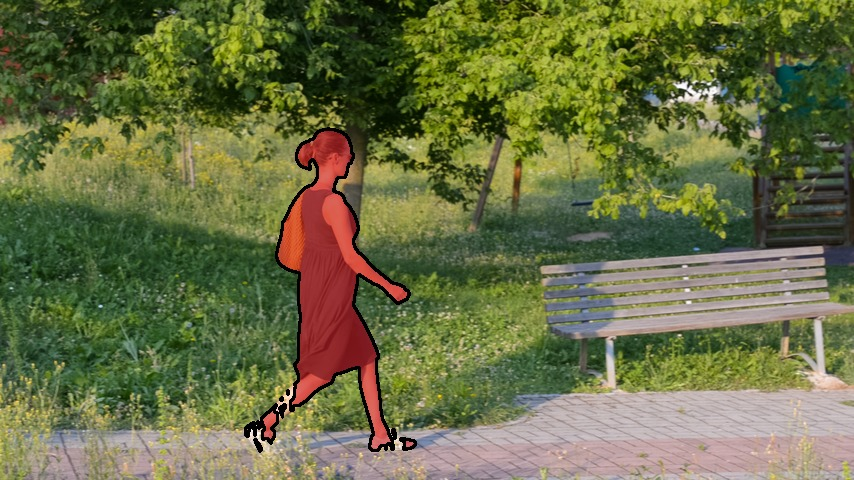
\includegraphics[width=0.3\columnwidth]{img/deconvLSTM/davis1.jpg}
    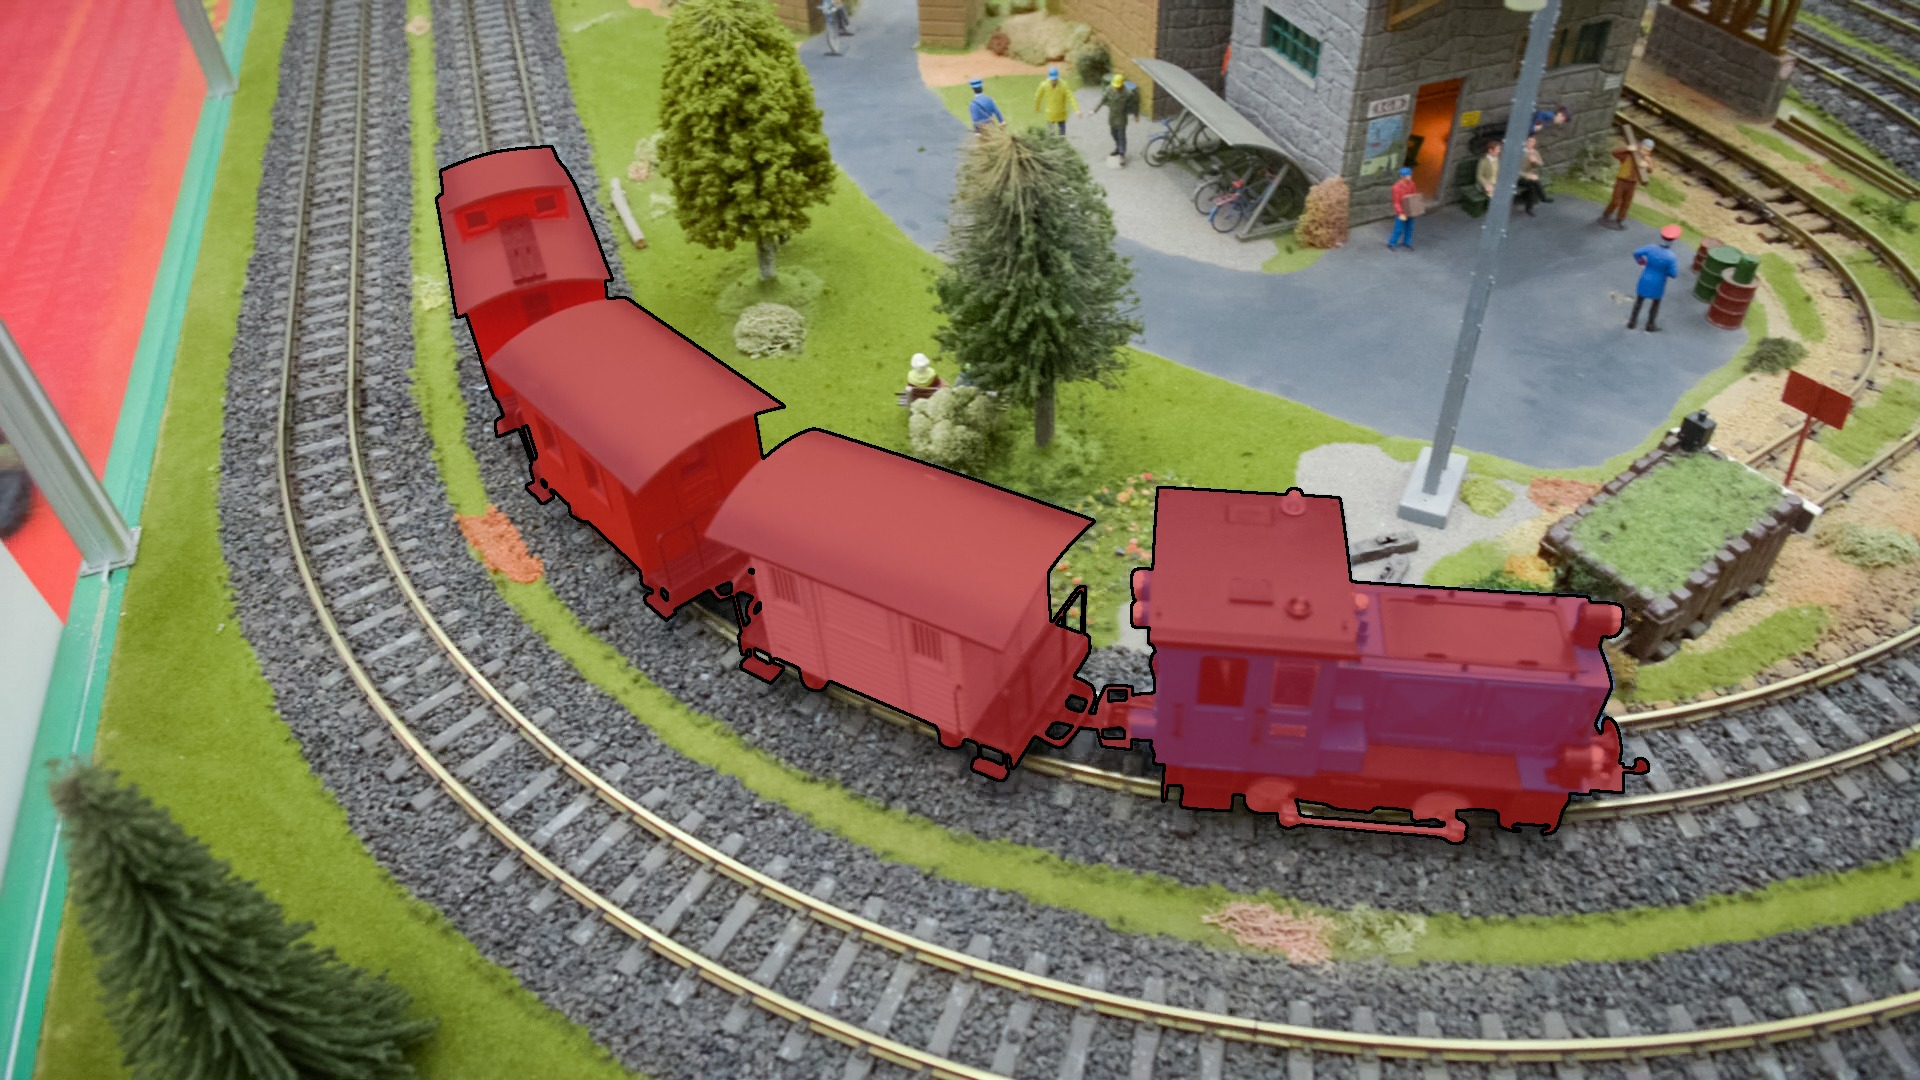
\includegraphics[width=0.3\columnwidth]{img/deconvLSTM/davis2.jpg}
    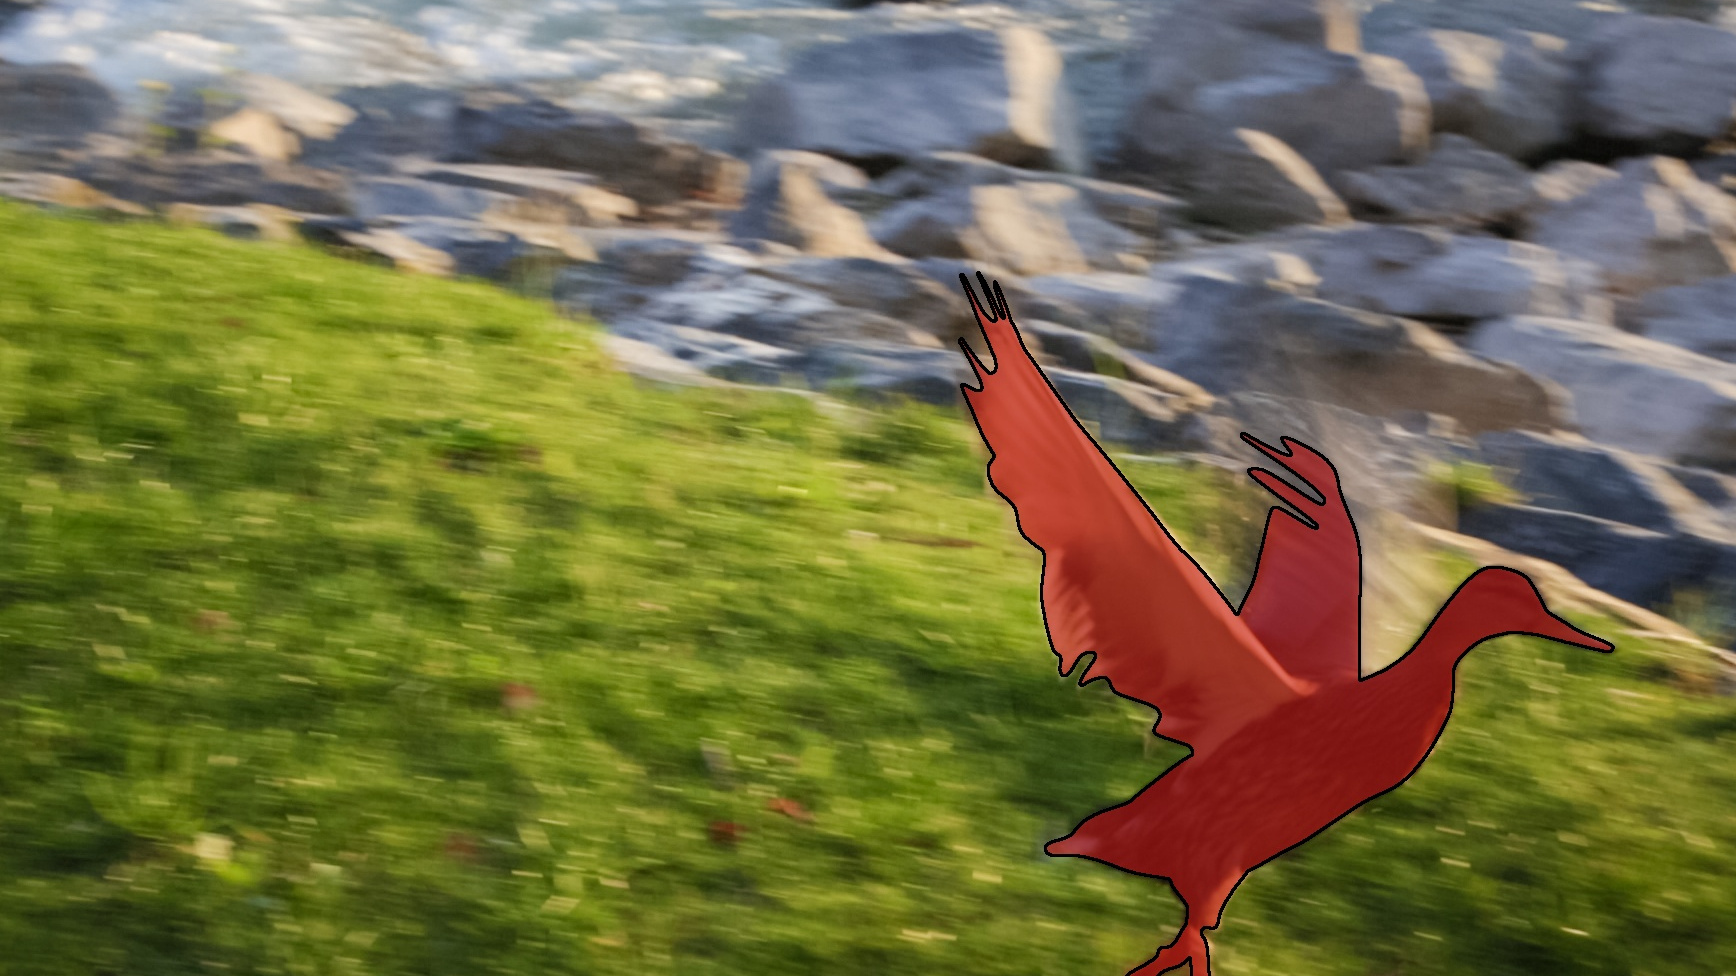
\includegraphics[width=0.3\columnwidth]{img/deconvLSTM/davis3.jpg}\\
    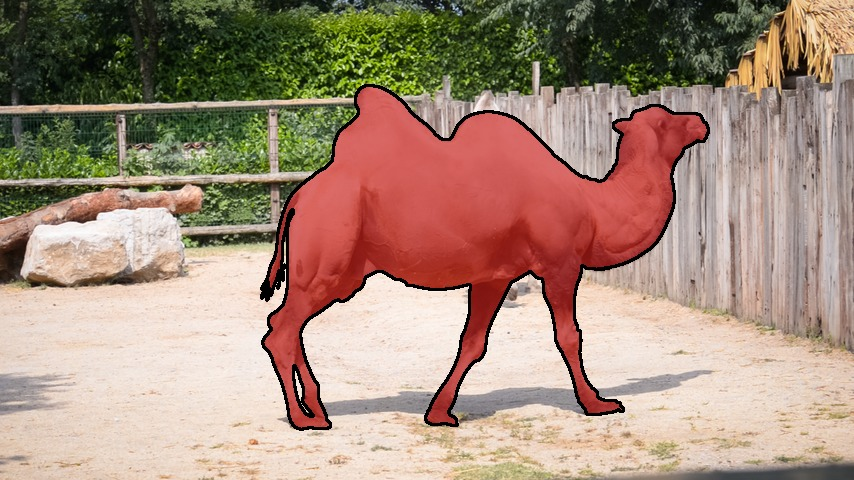
\includegraphics[width=0.3\columnwidth]{img/deconvLSTM/davis4.jpg}
    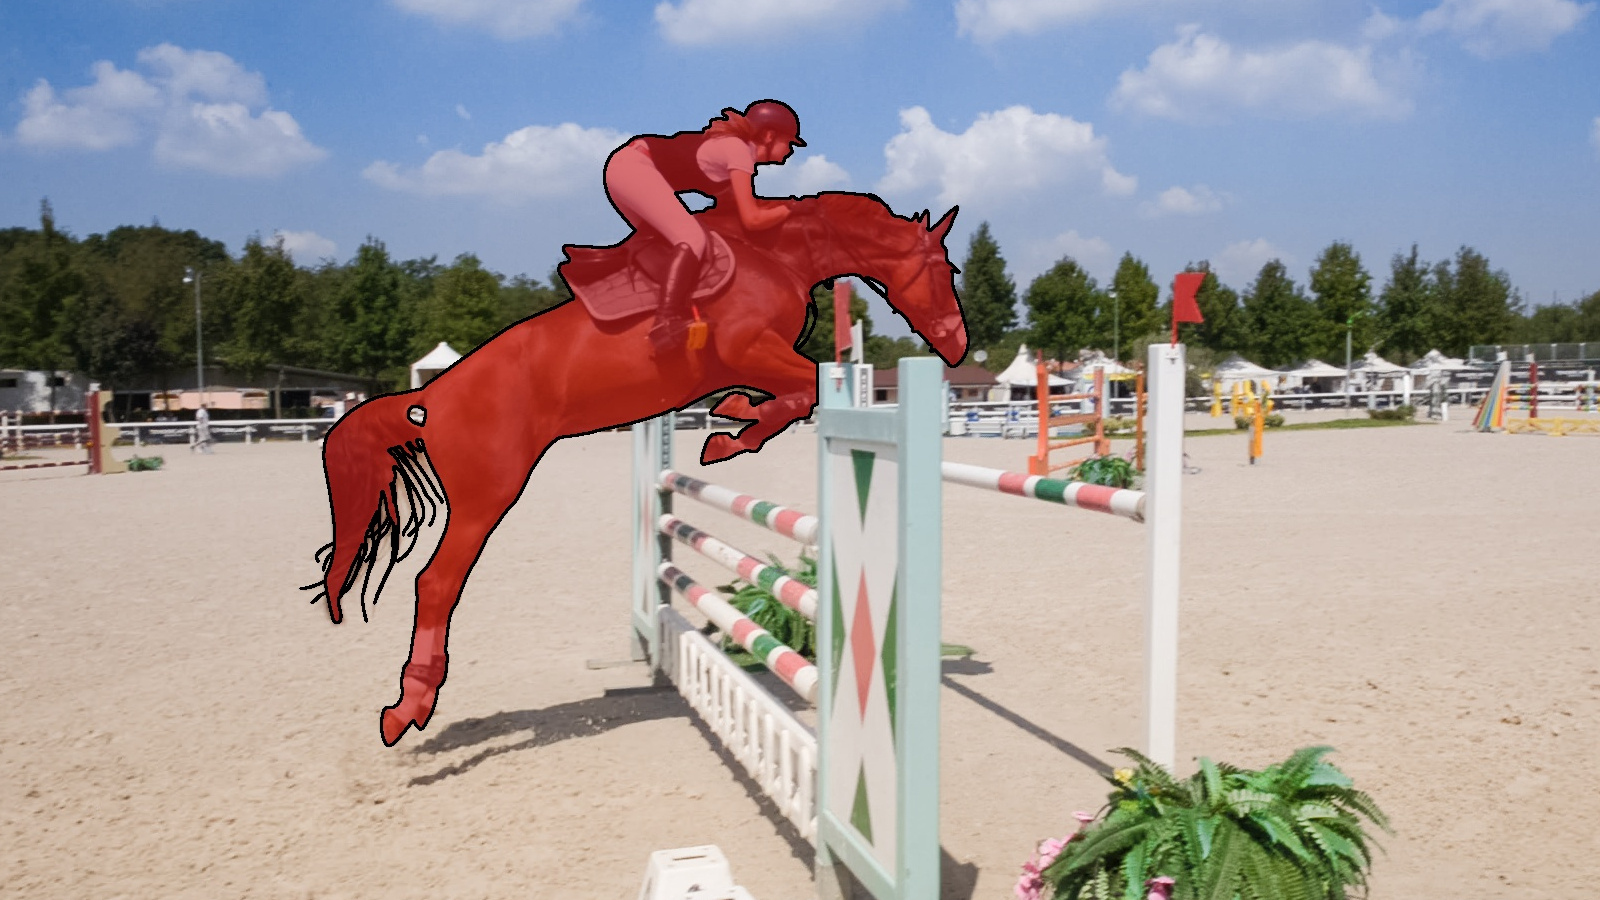
\includegraphics[width=0.3\columnwidth]{img/deconvLSTM/davis5.jpg}
    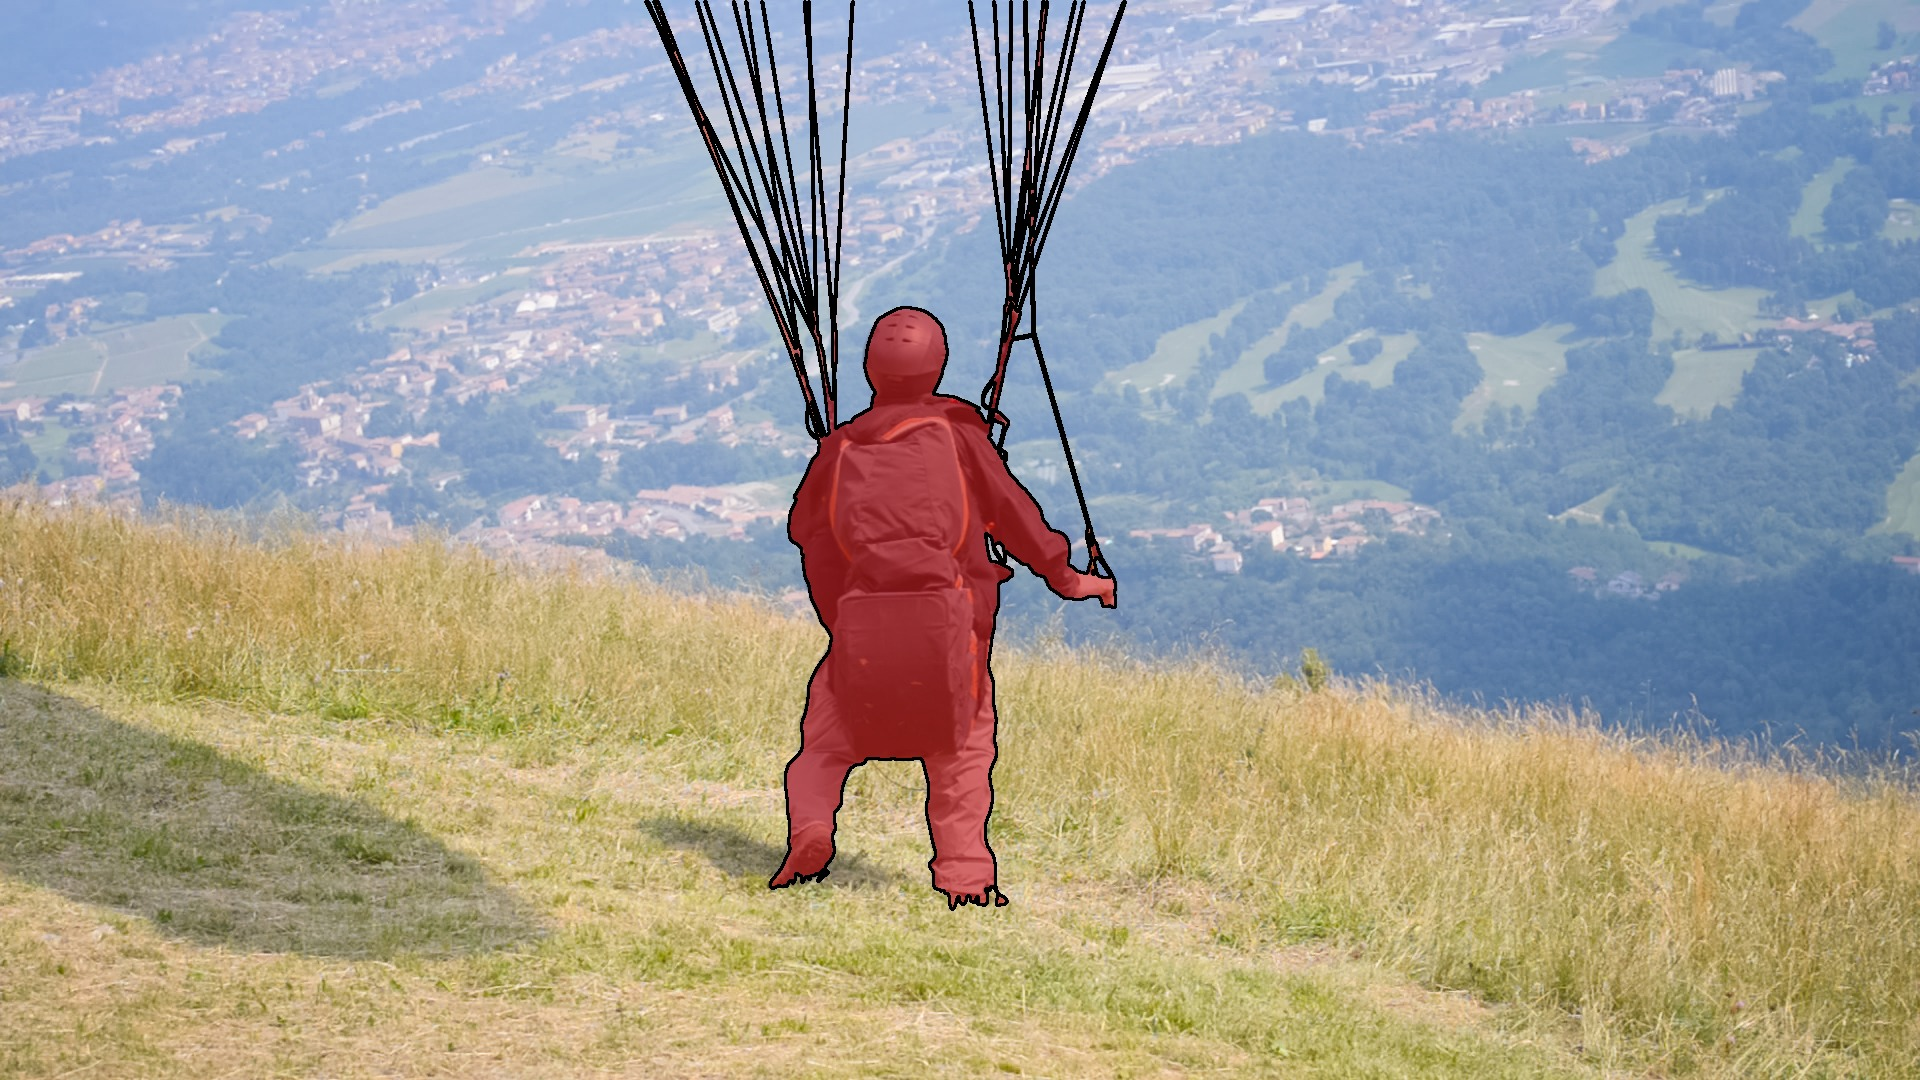
\includegraphics[width=0.3\columnwidth]{img/deconvLSTM/davis6.jpg}\\
    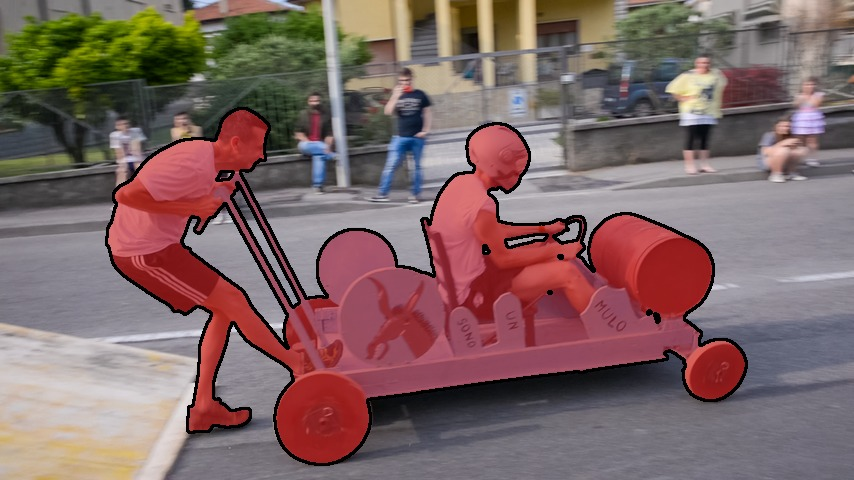
\includegraphics[width=0.3\columnwidth]{img/deconvLSTM/davis7.jpg}
    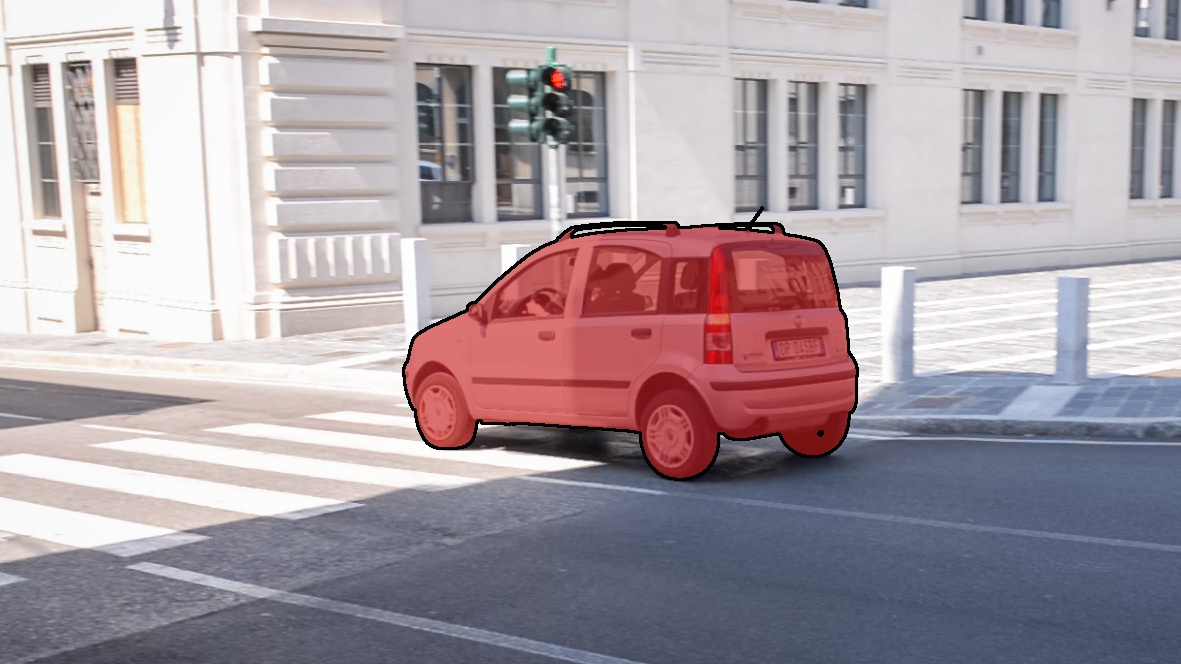
\includegraphics[width=0.3\columnwidth]{img/deconvLSTM/davis8.jpg}
    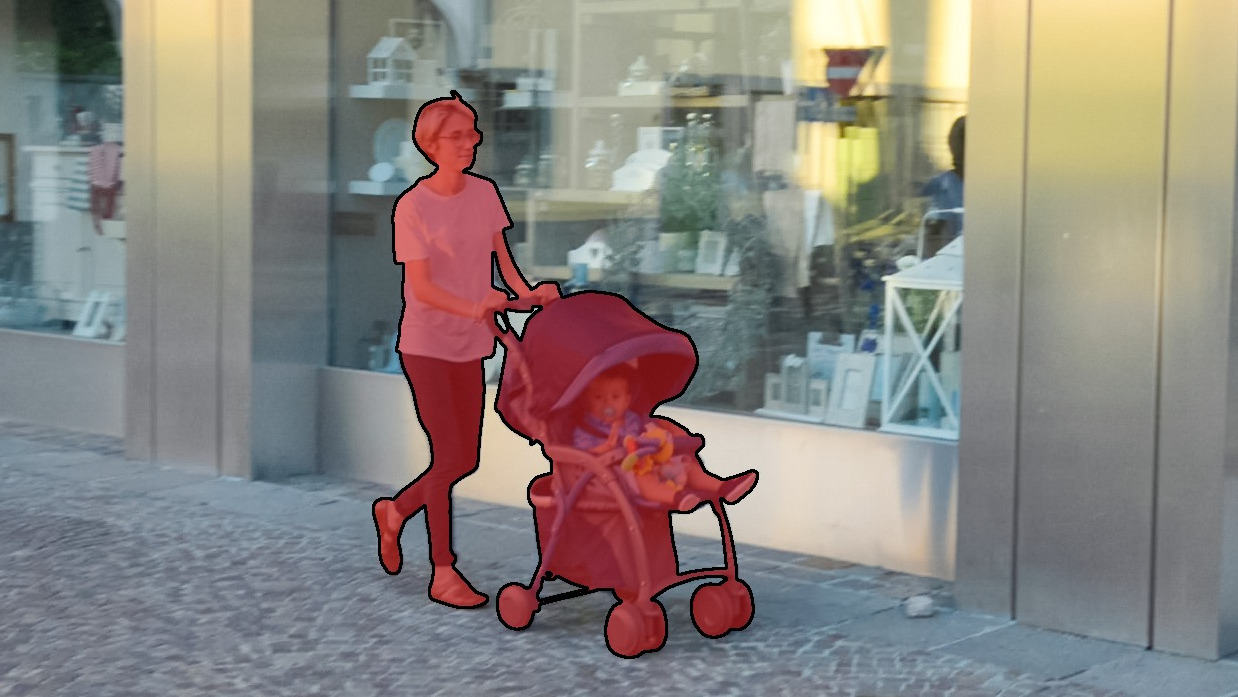
\includegraphics[width=0.3\columnwidth]{img/deconvLSTM/davis9.jpg}\\
    \caption{An example of ground truth segmentation for the DAVIS dataset.}
    \label{fig:deconvlstm_davis}
\end{figure}



% \subsubsection{Change Detection}
% \label{sssec:changedet}
% Change Detection dataset (CDnet) comes after 2 successful benchmarks
% \cite{wang2014cdnet,goyette2012changedetection}. CDnet contains over 160,000
% frames obtained from 31 videos and manually annotated. This dataset covers a
% variety of semantic segmentation scenarios. The categories include Challenging
% weather, Air turbulence, camera jitter, dynamic background, low resolution
% traffic videos, intermittent object motion, shadow, thermal, bad weather, low
% frame rate, night videos, pan-tilt-zoom and turbulence. The official evaluation
% metrics are Recall (Re), Specificity (Sp), False Positive Rate (FPR), False
% Negative Rate (FNR), Percentage of Wrong Classifications (PWC), Precision (Pr)
% and F-Measure (FM).


\subsection{Data augmentation and preprocessing}
%it has affine transformation, flipping, cropping, warping, etc...
Training on video semantic segmentation datasets is very time consuming, in
fact the prediction of a segmentation mask requires to densely process a
temporal window for each frame. This limits the size of the batches that can
be processed and slows down training.

With the goal of collecting a preliminary assessment of the performance of the
model and of its flexibility in tackling different kinds of datasets, it was
chosen to keep the training time as contained as possible without resorting to
data augmentation techniques. However, it has to be pointed out that some
degree of improvement can be expected from the introduction of some data
augmentation, e.g., by distorting the frames with affine transformations or by
flipping and rotating them.

In the same spirit, the only preprocessing technique adopted -- apart from
resizing the videos to allow a comparison with the state-of-the-art
(see~\autoref{sec:deconvLSTM_datasets}) -- was to normalize them frame-wise by
removing their mean and dividing by their standard deviation.

\subsection{Experimental settings}\label{sec:deconvLSTM_settings}
% In this section, we study the effectiveness of involving the temporal
% information on the task of video spatial segmentation. Our experiments with
% regarding to our pipeline are designed to find an optimum way of involving the
% temporal information.
% Toward this end, we compare our end to end segmentation method with two
% following baselines:
% \begin{itemize}
%     \item Segmentation over each frame independently using CNNs. In this
%         case, we don't involve any temporal information.
%     \item Employing the temporal information only on half of the network. (TODO:
%         why are we using this as a baseline?)
% \end{itemize}
% As explained earlier we employ the temporal information on every layers of the
% network and have a recursion over time at each layer. Therefore, we have both
% convolutional LSTM and upsampling LSTM. (TODO: requires more explanation)

% \subsubsection{Configuration of the layers}
% The convolutional and upsampling layers respectively consist of 70 and 100
% units. We apply batch normalization on each scale.
A first exploratory phase allowed to test several different architectures on
the relatively fast CamVid dataset and select a suitable starting point for the
rest of the experiments. The main hyperparameters of the DEConvLSTM model are
the number of encoding and decoding layers, as well as the depth of their inner
convolutions. As explained in~\autoref{sec:deconvLSTM_skip_connections}, it has
been chosen by design to constrain the number of decoding layers to be the same
as the number of encoding layers, to allow for the skip connections structure
to be symmetrical w.r.t. the middle feature map resolution of the network. The
number of such layers that empirically appeared to be optimal is 5, and has
been used consistently throughout the experiments.

Similarly, the number of inner convolutions and transposed convolutions has
been set to 2 (per layer) and their hyperparameters -- namely the number of
filters per sublayer~(\textbf{nf}), filters size per sublayer~(\textbf{fs}) and
stride per sublayer~(\textbf{st}) -- have been fixed as per~\autoref{%
tbl:deconvLSTM_enc_hyperparams} and \autoref{tbl:deconvLSTM_dec_hyperparams}.

\begin{table}[t]
    \centering{
        \small
        \begin{tabular}{c|c|c|c|c|c}
            \textbf{Layers} & 1 & 2 & 3 & 4 & 5\\ \hline
            \textbf{nf} & [64, 64] & [128, 128] & [256, 256] & [384, 384] &
                [512, 512]\\
            \textbf{fs} & [1x1, 3x3] & [1x1, 3x3] & [1x1, 3x3] & [1x1, 3x3] &
                [1x1, 3x3]\\
            \textbf{st} & [2, 2] & [2, 2] & [2, 2] & [2, 2] & [2, 2]\\
        \end{tabular}
    }
    \caption{ConvLSTM hyperparameters. Number of filters per
        sublayer~(\textbf{nf}), filters size per sublayer~(\textbf{fs}) and
        stride per sublayer~(\textbf{st}).}
    \label{tbl:deconvLSTM_enc_hyperparams}
\end{table}

\begin{table}[t]
    \centering{
        \small
        \begin{tabular}{c|c|c|c|c|c}
            \textbf{Layers} & 1 & 2 & 3 & 4 & 5\\ \hline
            \textbf{nf} & [384, 384] & [256, 256] & [128, 128] & [64, 64] &
                [64, 64]\\
            \textbf{fs} & [1x1, 3x3] & [1x1, 3x3] & [1x1, 3x3] & [1x1, 3x3] &
                [1x1, 3x3]\\
            \textbf{st} & [2, 2] & [2, 2] & [2, 2] & [2, 2] & [2, 2]\\
        \end{tabular}
    }
    \caption{TransConvLSTM hyperparameters. Number of filters per
        sublayer~(\textbf{nf}), filters size per sublayer~(\textbf{fs}) and
        stride per sublayer~(\textbf{st}).}
    \label{tbl:deconvLSTM_dec_hyperparams}
\end{table}

Throughout the experiments a light Dropout~\cite{Srivastava14} with drop
probability $0.2$ was used as regularization technique, as well as a
regularization of magnitude $0.0001$ for both the neural network weights and
the batch normalization. Optimization was carried on with
RMSProp~\cite{tieleman2012lecture} with learning rate $1e^{-4}$ and gradient
clipping of $10$. Finally, feature-wise batch normalization was applied before
each layer with an amount of momentum that varied from dataset to dataset.


\subsection{Results}\label{sec:deconvLSTM_results}

\autoref{tbl:deconvLSTM_camvid} reports the results on the Camvid dataset. All
the experiments were run with batch size $5$ training on cropped patches of
$224 \times 224$. The learning procedure was interrupted with early stopping on
the average Intersection over Union (IoU) of the validation set.
\autoref{tbl:deconvLSTM_camvid_overfit} reports the results of the preliminary
experiments on Camvid to assess the effect of different optimizers and various
sequence lengths. The models overfits heavily when the time correlation is
taken into account. This can be justified by some of the properties of the
dataset, as will be discussed in~\autoref{sec:deconvLSTM_discussion}.

\begin{table}[t]
    \centering{\small
        \begin{tabular}{l|c||c}
            Method & Global accuracy & \textbf{Avg IoU}\\ \hline

            SegNet-Basic \cite{badrinarayanan2015segnet} & 82.8 & 46.3 \\
            SegNet \cite{badrinarayanan2015segnet} &  88.6 & 50.2 \\
            ReSeg \cite{Visin_2016_CVPR_Workshops} & 88.7 & 58.8 \\
            Dilation \cite{yu2015multi} & n/a & 65.3 \\
            Dilation + FSO - DiscreteFlow \cite{kundu2016feature} & n/a & 66.1 \\
            DEConvLSTM (sequence length = 3) & 78.8 & 38.2
        \end{tabular}
    }
    \caption{Results on the CamVid dataset. Pixel accuracy and average
        Intersection over Union (IoU) are reported.}
    \label{tbl:deconvLSTM_camvid}
\end{table}

\begin{table}[t]
    \centering{\small
        \begin{tabular}{c|c|c|c|c|c|c|c}
            & & \multicolumn{3}{c}{Global accuracy} & \multicolumn{3}{c}{\textbf{Avg IoU}}\\
            Optimizer & Sequence length & Test & Validation & Train & Test & Validation & Train\\ \hline
            RMSProp & 3 & 78.0 & 37.8 & 90.2 & 58.4 & 91.5 & 60.3\\
            Adam & 3 & 78.8 & 38.2 & 90.3 & 58.3 & 91.4 & 59.8\\
            RMSProp & 1 & 83.1 & 46.6 & ? & ? & ? & ?
        \end{tabular}
    }
    \caption{Preliminary experiments on the CamVid dataset. Pixel accuracy and
        average Intersection over Union (IoU) are reported. Overfitting is very
        strong when temporal correlation is exploited.}
    \label{tbl:deconvLSTM_camvid_overfit}
\end{table}

% ADAM seq_len 3
% =============================
% test_acc: 0.788309417551
% test_jaccard: 0.38183944114
% valid_acc: 0.903313517338
% valid_jaccard: 0.582879679893
% train_acc: 0.914322370271
% train_jaccard: 0.597896683484

% RMSProp seq_len 3
% =============================
% test_acc: 0.780264451
% test_jaccard: 0.377975928479
% valid_acc: 0.901692251912
% valid_jaccard: 0.58374693901
% train_acc: 0.915286386415
% train_jaccard: 0.602986412809

\autoref{tbl:deconvLSTM_camvid} reports the results of the DEConvLSTM model on
the Gatech Dataset. Remarkably, the performance of the DEConvLSTM model on this
dataset aligns to the state-of-the-art. As discussed before, many modifications
(such as data augmentation) can be adopted to increase the performance of the
model and fully set the state-of-the-art. The focus of the research carried on
on this model so far has been mainly to evaluate the proposed architecture in
non-trivial settings where the time component can be exploited to improve the
prediction of the model. However as future steps we intend to run more
experiments with the goal to set a new state-of-the-art.


\begin{table}[t]
    \centering{\small
        \begin{tabular}{l||c}
            Method & \textbf{Global accuracy}\\ \hline

            2D-V2V \cite{Tran16v2v} & 55.7 \\
            V2V-0 \cite{Tran16v2v} & 66.7 \\
            Conv3b + Up \cite{Tran16v2v} & 69.7 \\
            Conv4b + Up \cite{Tran16v2v} & 72.7 \\
            Conv5b + Up \cite{Tran16v2v} & 72.1 \\
            \textbf{V2V} \cite{Tran16v2v} & \textbf{76.0} \\
            \textbf{DEConvLSTM} & \textbf{76.1}
        \end{tabular}
    }
    \caption{Results on the Gatech dataset. Pixel accuracy is reported.}
    \label{tbl:deconvLSTM_gatech}
\end{table}

%have 80% + of accuracy in val in gatech
% 46 epochs, val loss 0.4873, val jacquard 0.4865...
% Epoch 53/300 - loss: 0.2103 - cat_masked_accuracy: 0.9281 - val_loss: 0.3016 - val_jaccard: 0.6224

Finally, \autoref{tbl:deconvLSTM_davis} reports the initial results of the
DEConvLSTM model on the Davis Dataset. This early encouraging result calls for
more thorough experiments on this dataset.

\begin{table}[t]
    \centering{\small
        \begin{tabular}{l||c}
            Method & \textbf{Avg IoU}\\ \hline

            Temporal superpixels \cite{chang2013video} & 35.8 \\
            SeamSeg \cite{ramakanth2014seamseg} & 55.6 \\
            Efficient hierarchical graph-based video segmentation \cite{
                grundmann2010efficient} & 59.6 \\
            Jumpcut \cite{fan2015jumpcut} & 60.7 \\
            Fully Connected Object Proposals for Video Segmentation \cite{
                perazzi2015fully} & 63.1 \\
            \textbf{Bilateral space video segmentation} \cite{
                marki2016bilateral} & 66.5 \\
            DEConvLSTM & 56.8
        \end{tabular}
    }
    \caption{Results on the Davis dataset. Average Intersection over Union
        (IoU) is reported.}
    \label{tbl:deconvLSTM_davis}
\end{table}


\section{Discussion}\label{sec:deconvLSTM_discussion}
One of the first goals of the experiments with the DEConvLSTM model was to
assess the effectiveness of exploiting the temporal correlation among frames in
the task of video spatial segmentation. To this end several tests were run on
CamVid, training the same model varying the length of the sequence.

CamVid has been mostly used in the literature in a single image
segmentation setting, rather than considering the frames altogether as a video.
Indeed, on this dataset the model performed better when the sequence length was
set to 1, i.e., when the temporal correlation was not taken into account.
This is not too surprising, since this dataset is composed by frames captured
at 30 fps, but only one frame out of approximately 30 is annotated and available
for training. The experiments show that trying to exploit temporal correlation
at 1 Hz is very non-trivial, and results in massive overfitting.

Overfitting is an important problem when training on the CamVid dataset, since
the training set is relatively small for a big model like DEConvLSTM. In
particular the performance comparison between different lengths of the input
sequences highlights a strong tendency of the network to overfit on longer
sequences, as shown in~\autoref{tbl:deconvLSTM_camvid_overfit}. TODO is this true??

On the contrary, there is evidence in the literature that exploiting the
temporal correlation between frames improves performance on Gatech~\cite{
Tran16v2v} so no test was performed in this direction on this dataset. The
results reported in \autoref{tbl:deconvLSTM_gatech} show the interesting
potential of the DEConvLSTM model on the video semantic segmentation task.

Unfortunately the model did not range as well on the Davis dataset. The failure
mode in this case seems to be the task itself: the algorithm is expected to
segment the only main element in the scene. Apparently the network struggles
identifying what to segment and what not to and ends up focusing too much on
the background, heavily decreasing the segmentation performances.

One interesting discovery is that using the per-batch statistics at training as
well as at test time (rather than the more common strategy of re-using the
training running statistics at test time) significantly improved the results on
all the three datasets. Another crucial factor to achieve a good optimization
is to select the right amount of momentum in the computation of the batch
normalization statistics. We argue that this the reason for both behaviors lies
in the high variance of the input data. The datasets are in fact composed by
sequences of frames coming from different videos that can vary consistently in
terms of e.g. brightness, scale and noise. Relying too heavily on past
statistics in this setting can be harmful.

Video semantic segmentation is a hard task to tackle. CNNs are known to be
data hungry, as proved by the great performance leap that followed the
introduction of large dataset for object classification~\citep{ILSVRCarxiv14}.
The next milestone for computer vision research is reaching a good
understanding of videos in structured prediction related tasks. Good datasets
with large amounts of densely annotated video data are still missing, even if
the community is making an effort to fill in the gap~\citep[see~e.g.,~][]{
Perazzi2016}. Nonetheless it is already possible to challenge non-neural
methods and reach reasonable results - when not state-of-the-art performances.
More work is needed to speed up the models, study new loss functions that allow
to optimize more closely non-derivable metrics such as IoU, reuse computation
exploiting similarity in consecutive frames. Coupling CNNs, transposed CNNs
and LSTMs can be an effective way to tackle structured prediction problems in
video, building on the speed of CNNs to process spacial information and on the
ability of RNNs to retain information through several steps of computation.


%to handle variable size images we could just have used something like SPP
% the argument is that TIME really has to make a difference
% it is just that we need more data
% and show that some results are reasonable
% although not SOTA
% and the next big step is video
%FCN8, FCN8 with convLSTM, our model

%/data/lisa/exp/romerosa/deconvRNN/tmp/
%/data/lisatmp4/romerosa/deconvRNN

